\documentclass[aspectratio=43]{beamer}
% !TeX document-id = {2870843d-1baa-4f6a-bd0a-a5c796104a32}
% !BIB TS-program = biber
% !TeX encoding = UTF-8
% TU Delft beamer template

\documentclass[aspectratio=43]{beamer}
\usepackage[english]{babel}
\usepackage{csquotes}
\usepackage{calc}
\usepackage[absolute,overlay]{textpos}
\usepackage{graphicx}
\usepackage{subfig}
\usepackage{mathtools}
\usepackage{amsfonts}
\usepackage{amsthm}
\usepackage{comment}
\usepackage{siunitx}
\usepackage{MnSymbol,wasysym}
\usepackage{array}
\usepackage{qrcode}

\setbeamertemplate{navigation symbols}{} % remove navigation symbols
\mode<presentation>{\usetheme[verticalbar=false]{tud}}

% BIB SETTINGS
\usepackage[
    backend=biber,
    giveninits=true,
    maxnames=30,
    maxcitenames=20,
    uniquename=init,
    url=false,
    style=authoryear,
]{biblatex}
\addbibresource{bibfile.bib}
\setlength\bibitemsep{0.3cm} % space between entries in the reference list
\renewcommand{\bibfont}{\normalfont\scriptsize}
\setbeamerfont{footnote}{size=\tiny}
\renewcommand{\cite}[1]{\footnote<.->[frame]{\fullcite{#1}}}
\setlength{\TPHorizModule}{\paperwidth}
\setlength{\TPVertModule}{\paperheight}

\newcommand{\absimage}[4][0.5,0.5]{%w
	\begin{textblock}{#3}%width
		[#1]% alignment anchor within image (centered by default)
		(#2)% position on the page (origin is top left)
		\includegraphics[width=#3\paperwidth]{#4}%
\end{textblock}}

\newcommand{\mininomen}[2][1]{{\let\thefootnote\relax%
	\footnotetext{\begin{tabular}{*{#1}{@{\!}>{\centering\arraybackslash}p{1em}@{\;}p{\textwidth/#1-2em}}}%
	#2\end{tabular}}}}
%% Useful example slides 
%\section{Introduction}
{
\setbeamertemplate{footline}{\usebeamertemplate*{minimal footline}}
\frame{\titlepage}
}

% \begin{frame}[fragile]{Example frame 1} % some commands, e.g. \verb require [fragile]
    This is the first frame.
    
    You can set the blue bar vertical using the option \verb|\usetheme[verticalbar=true]{tud}|.
    
    Set the aspect ratio to 4:3 with the
    documentclass option aspectratio=43. Use aspectratio=169 for wide screen (16:9).
    \end{frame}
% \section{Examples}
\begin{frame}{Example frame 2}
  \begin{block}{Block}
    \begin{itemize}
      \item item 1
      \item item 2
    \end{itemize}
  \end{block}

  \begin{exampleblock}{Example}
    \begin{enumerate}
      \item Sugar in a stirred cup of tea gathers in the middle.
      \item Rivers often take a detour through flat terrain.
    \end{enumerate}
  \end{exampleblock}

  \begin{alertblock}{Alert}
     Rivers and sweet tea do unexpected things.\cite{Einstein1926}
  \end{alertblock}
\end{frame}
% \begin{frame}{Mass--energy equivalence}
	They say every formula you add to a presentation, will reduce your audience by \SI{50}{\percent}. A simple yet effective way to mitigate this effect, is adding a compact nomenclature to the slides containing formulae.
	
	\[E=mc^2\]
	
	If you find this is taking up too much of your precious space, than you are doing something wrong, and it is not adding this little nomenclature.
	
	The optional argument specifies the number of column pairs.
	
\mininomen[2]{% number of columns
  $E$ & Energy (\unit{J})                     & $m$ & Mass (\unit{kg}) \\
  $c$ & Speed of light in vacuum (\unit{m/s}) \\[2ex] % may need some tweaking
  }
\end{frame}
% \input{sections/examples/columnslide.tex}
% 
\section{Conclusion}
\begin{frame}[fragile]{animation}
  \vfill
  Some commands take optional arguments in the form of \verb|<x-y>|,
  where \verb|x| is the first `sub-frame' on which the context is shown,
  and \verb|y| is the last. \verb|x| or \verb|y| can be replaced by \verb|+|,
  referring to `the next sub-frame'. 
  \vfill
  \begin{columns}[onlytextwidth]
  \begin{column}{.5\textwidth}
    \begin{enumerate}
      \item<+-> uncovered\ldots
      \item<+-> one\ldots
      \item<+-> by\ldots
      \item<+-> one.
    \end{enumerate}
    \end{column}
  \begin{column}{.5\textwidth}
      Using only:\only<1>{1}\only<2>{2}\only<3>{3}

      Using onslide:\onslide<1>{1}\onslide<2>{2}\onslide<3>{3}

      Using pause:\pause1\pause2\pause3
  \end{column}
  \end{columns}
  \vfill
  For more advanced animations, see \S 14 of the manual:\\
  \url{https://www.ctan.org/pkg/beamer}
  % \url{https://www.ctan.org/pkg/animate}\\
  % \url{https://www.ctan.org/pkg/media9}
  \vfill
  % \transduration{2} automatic progression of slides
  \transpush<1>
\end{frame}
% \begin{frame}
    Thanks for your attention.
  
    A digital version of this presentation can be found here:
    \vfill
    \url{https://gitlab.com/novanext/tudelft-beamer} 
    \vfill  
    \centering
    \qrcode{https://gitlab.com/novanext/tudelft-beamer}
    \vfill
  \end{frame}
% \begin{frame}[allowframebreaks,t]{\bibname}
	% the 'I' is caused by 'allowframebreaks'
	\AtNextBibliography{\footnotesize}% or in the preamble \AtBeginBibliography{\small}
	\printbibliography
\end{frame}


%% Our presentation

\title[]{Improving Digital Twin of STEDIN Transformer}
\institute[]{Delft University of Technology, The Netherlands}
\author{Auke Schaap \and Philip Soliman}
\date{}


\begin{document}
\section{Introduction}
{
\setbeamertemplate{footline}{\usebeamertemplate*{minimal footline}}
\frame{\titlepage}
}

\section{Stedin & Transformers}
\begin{frame}[fragile]{Transformer} % some commands, e.g. \verb require [fragile]
\begin{figure}
    \centering
    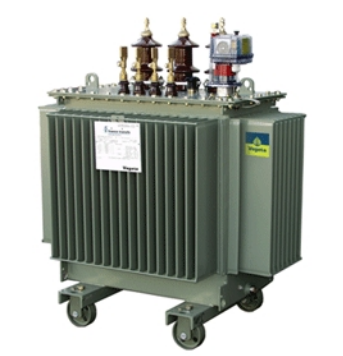
\includegraphics[width=0.6\textwidth]{figures/transformer.png}
    \label{fig:my_label1}
\end{figure}
\end{frame}

\begin{frame}[fragile]{Distribution grid} % some commands, e.g. \verb require [fragile]
\begin{figure}
    \centering
    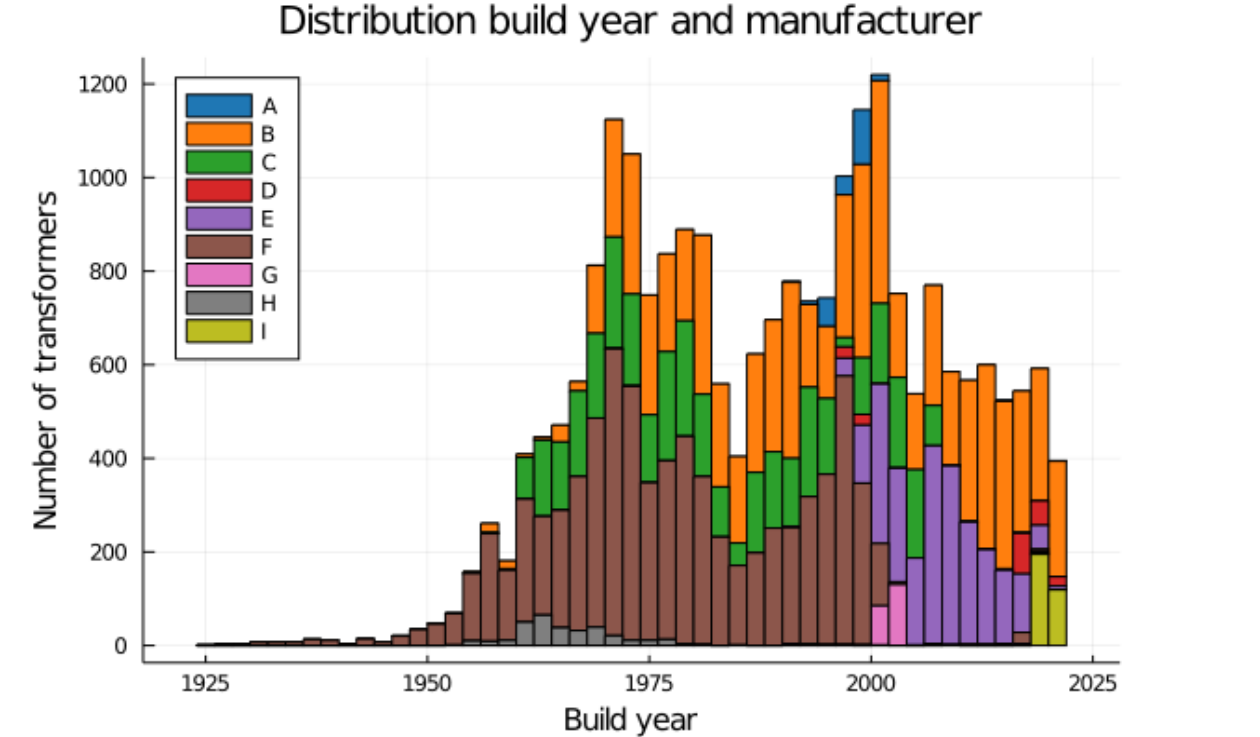
\includegraphics[width=0.9\textwidth]{figures/stedin_transformers_build_year.png}
    \label{fig:my_label2}
\end{figure}
\end{frame}

\begin{frame}[fragile]{Distribution grid} % some commands, e.g. \verb require [fragile]
\begin{figure}
    \centering
    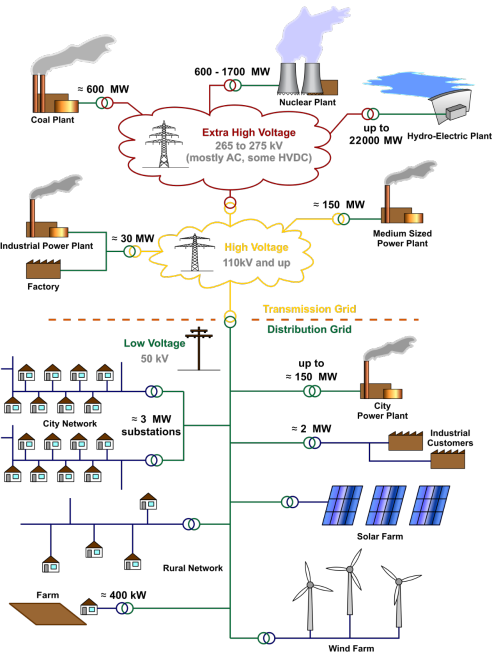
\includegraphics[width=0.5\textwidth]{figures/distribution grid.png}
    \label{fig:my_label3}
\end{figure}
\end{frame}

\begin{frame}[fragile]{Transformer Core} % some commands, e.g. \verb require [fragile]
\begin{figure}
    \centering
    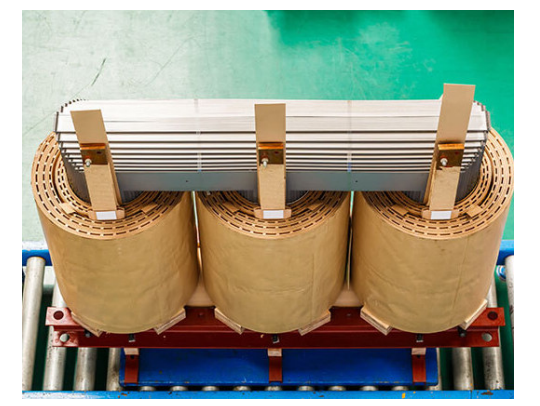
\includegraphics[width=0.8\textwidth]{figures/transformercore.png}
    \label{fig:my_label4}
\end{figure}
\end{frame}

\section{Derivation}
\begin{frame}{Derivation}
The Maxwell equations are given by
\begin{align*}
    \nabla \times \mathbf{E} &= -\frac{\partial \mathbf{B}}{\partial t}, \\
    \nabla \times \mathbf{H} &=  \mathbf{J} + \frac{\partial \mathbf{D}}{\partial t}, \\
    \nabla \cdot \mathbf{B} &= 0, \\
    \nabla \cdot \mathbf{D} &= \rho,
\end{align*}
where
\begin{itemize}
    \item $\mathbf{E}, [V/m]$ is the electric field intensity,
    \item $\mathbf{H}, [A/m]$ is the magnetic field intensity,
    \item $\mathbf{J}, [A/m^2]$ is the current density,
    \item $\mathbf{B}, [T]$ is the magnetic flux density,
    \item $\mathbf{D}, [C/m^2]$ is the electric flux density,
    \item $\rho, [C/m^3]$ is the free charge density.
\end{itemize}
\end{frame}


\begin{frame}{Derivation}
Using the potential formulation,
\begin{align*}
    \mathbf{E} &= -\nabla \varphi -\frac{\partial \mathbf{A}}{\partial t}, \\
    \mathbf{B} &= \nabla \times \mathbf A,
\end{align*}
we can formulate a system that we can solve.

\end{frame}

\begin{frame}{Derivation}

\begin{assumption}
    The permittivity of vacuum $\epsilon_0$ is very small, $(\mathcal{O}(10^{-12}))$, and for all materials in this research $\epsilon_r < 10$, so $\epsilon$ can be neclegted. Therefore, $\mathbf{D} = 0$ and can be neglected.
\end{assumption}

\begin{assumption}
    We assume that the contribution of the electrostatic field $\varphi$ is negligble compared to the contribution of the potential field $\mathbf A$. That is, $\nabla \varphi = 0$, which implies that $\mathbf{E} = -\frac{\partial \mathbf{A}}{\partial t}$.
\end{assumption}

\begin{assumption}
    The flow of current is oriented along the $z$ axis, and the geometry is in the $xy$ plane. That is, $\mathbf{A} = (0, 0, A_z)$ and $\mathbf{J_e} = (0, 0, J_z)$. This implies $\nabla \times \mathbf A = \nabla A_z$.
\end{assumption}
\end{frame}



\section{Definition}
\begin{frame}[fragile]{Definition} % some commands, e.g. \verb require [fragile]    
    \begin{problemdef}
        Find $A_z$ in the system
        \begin{equation}
            \sigma\frac{\partial A_z}{\partial t} = \nabla \times \left[\frac{1}{\mu}\nabla A_z\right] + J_z,
        \end{equation}
        where
        \begin{itemize}
            \item $A_z$ is the current density in the $z$ direction,
            \item $\mu$ is the permeability of the core,
            \item $J_z$ is the imposed source current density,
            \item $\sigma$ is the conductivity of the core.
        \end{itemize}
        From this point onwards, this will be formulated as
        \begin{equation}
            \sigma\dot u = \nabla \times \left[\frac{1}{\mu}\nabla u\right] + f.
        \end{equation}
    \end{problemdef}
\end{frame}


\section{Approaches}
\begin{frame}[fragile]{Approaches} % some commands, e.g. \verb require [fragile]

There are a couple of situations we could look at
\begin{itemize}
    \item Steady state ($\omega = 0$)
    \item Single frequency ($\omega = 50$)
    \item Multi frequency
    \begin{itemize}
        \item Linear
        \item Nonlinearities
    \end{itemize}
\end{itemize}
\end{frame}



\begin{frame}[fragile]{Approach I: Steady state} % some commands, e.g. \verb require [fragile]


\begin{discretization}
    \begin{equation*}
        0 = \frac{1}{\mu}K u + f,
    \end{equation*}
    where
    \begin{itemize}
        \item $u$ is $A_z$, the solution.
        \item $M$ is the mass matrix,
        \item $K$ is the stiffness matrix,
        \item $f$ is the source term, given by $J_z$,
    \end{itemize}
\end{discretization}
\end{frame}

\begin{frame}[fragile]{Steady State Solution} % some commands, e.g. \verb require [fragile]
\begin{figure}
    \centering
    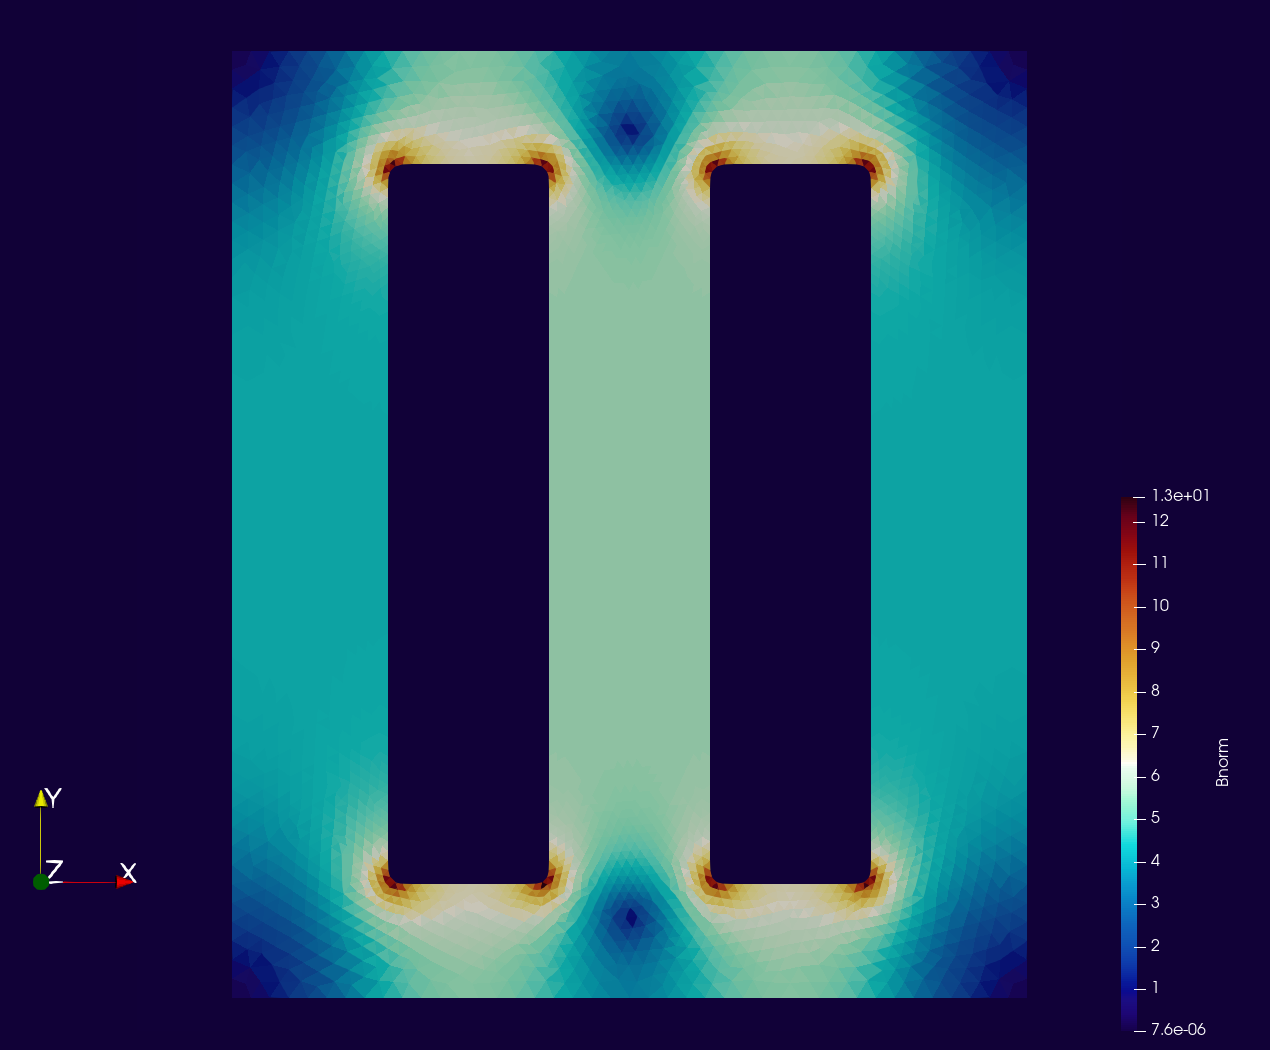
\includegraphics[width=0.8\textwidth]{figures/steady_state_cropped.png}
    \label{fig:my_label}
\end{figure}
\end{frame}

\begin{frame}[fragile]{Approach II: Single frequency} % some commands, e.g. \verb require [fragile]

We assume that there is only one frequency at play, thus there is separation of variables.
\begin{align*}
    u(x,y,t) = \hat u(x,y) \cdot e^{j\omega t}
\end{align*}

\begin{discretization}
    \begin{equation*}
        \sigma \omega j M u  = \frac{1}{\mu}K u + f,
    \end{equation*}
    where
    \begin{itemize}
        \item $u$ is $A_z$, the solution.
        \item $M$ is the mass matrix,
        \item $K$ is the stiffness matrix,
        \item $f$ is the source term, given by $J_z$,
    \end{itemize}
\end{discretization}
\end{frame}

% \begin{frame}[fragile]{Approach II: Single frequency}

% \begin{discretization}
%  \[A_z = \hat{A}_z(x,y)e^{i\omega t}, \]

% \[ -\nabla \times \left[\frac{1}{\mu}\nabla A_z\right] + i\sigma\omega A_z= \mathbf J_0, \]   

% \[
% \left(-K+i\omega M\right)u = f
% \]
% \end{discretization}
% \end{frame}


\begin{frame}[fragile]{Approach III: Multi-frequency} % some commands, e.g. \verb require [fragile]
\begin{discretization}
    \begin{equation*}
        \sigma M \dot u = \frac{1}{\mu}K u + f,
    \end{equation*}
    where
    \begin{itemize}
        \item $u$ is $A_z$, the solution.
        \item $M$ is the mass matrix,
        \item $K$ is the stiffness matrix,
        \item $f$ is the source term, given by $J_z$,
    \end{itemize}
\end{discretization}
We simply solve this system for each frequency and add up the result. 
\end{frame}

\begin{frame}[fragile]{BH curve \& non-linear materials}
  \begin{columns}[onlytextwidth]
    \begin{column}{.5\textwidth}
    Steady state solution assuming linear material
        \begin{figure}
            \centering
            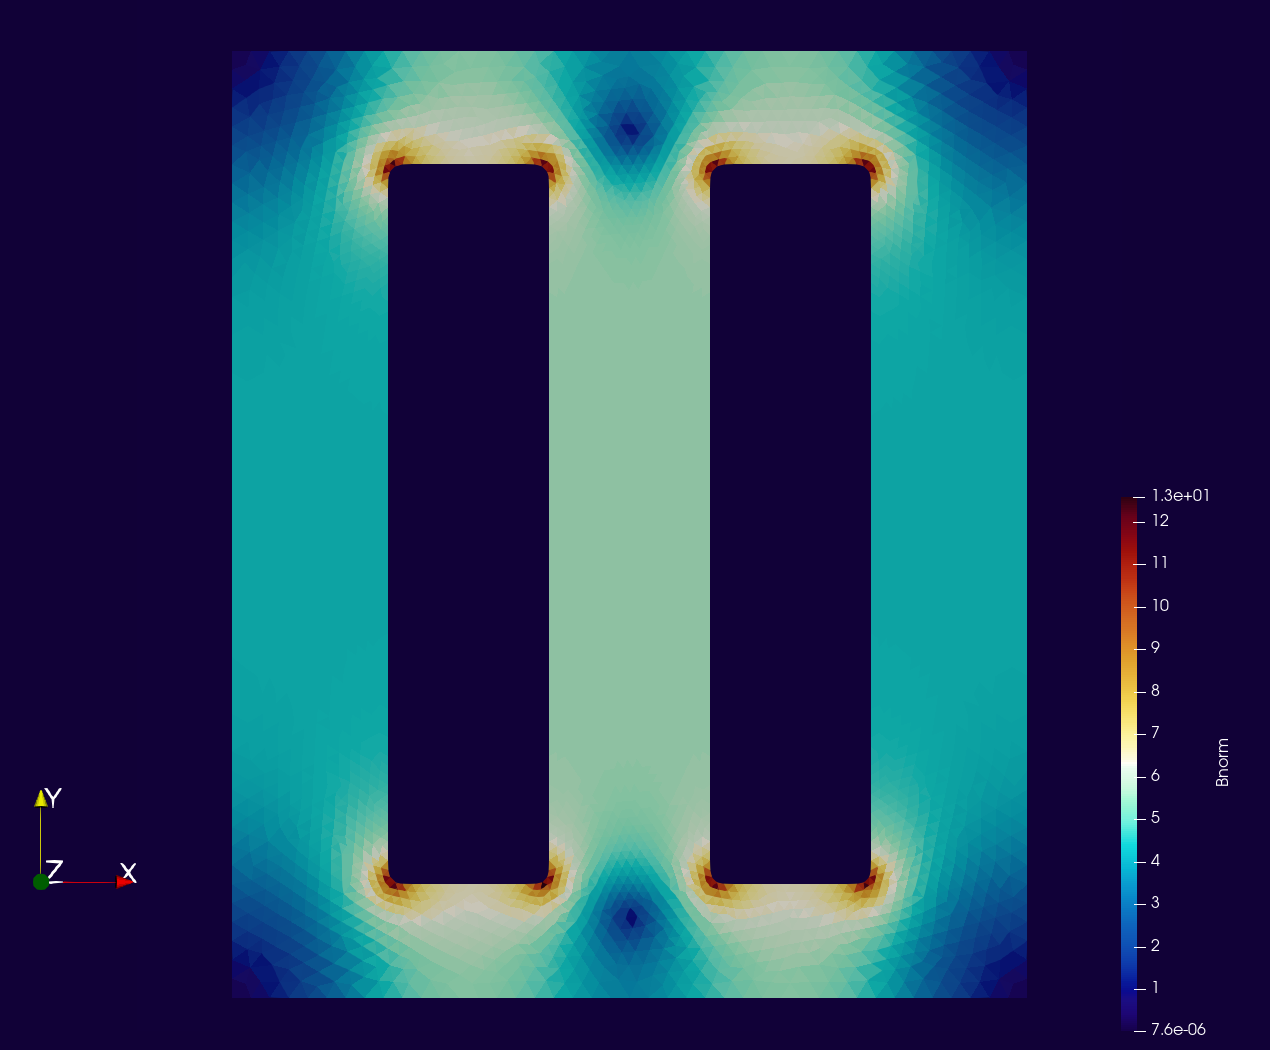
\includegraphics[width=1\textwidth]   {figures/steady_state_cropped.png}
            \label{fig:my_label}
        \end{figure}
    \end{column}
    \begin{column}{.5\textwidth}
    \quad BH curve. $\mu = \mu(||\nabla B||)$ 
        \begin{figure}
            \centering
            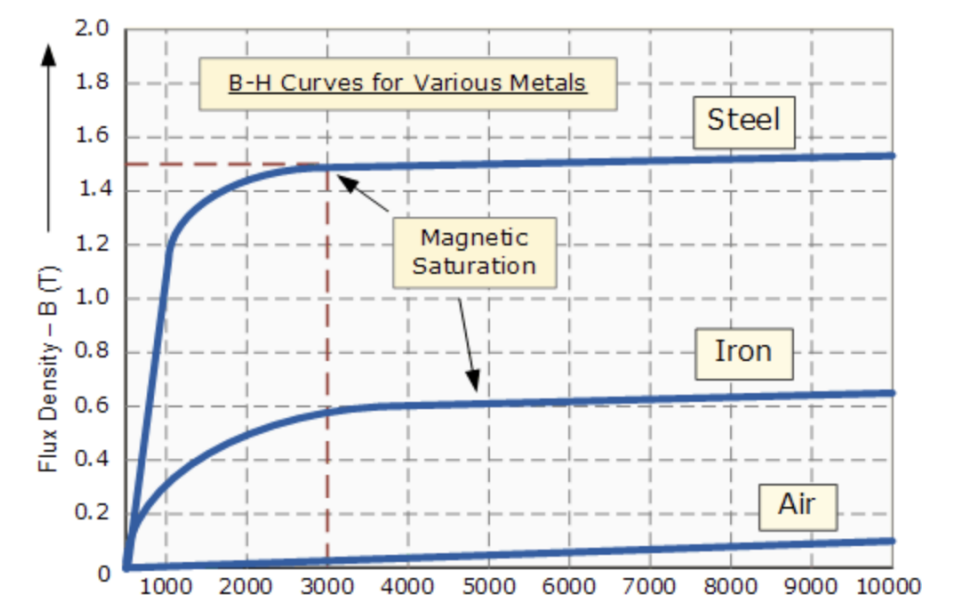
\includegraphics[width=1\textwidth]{figures/BH curve.png}
            \label{fig:my_label}
        \end{figure}
    Super Position is not allowed anymore!
    \end{column}
  \end{columns}
\end{frame}

\begin{frame}[fragile]{Further work} % some commands, e.g. \verb require [fragile]
\begin{itemize}
    \item Check superposition assumption
    \item Time stepping
    \item Optimizations
    \item Hybrid mesh for boundary layers
    
    
\end{itemize}
\end{frame}


\begin{frame}[fragile]{Questions?} % some commands, e.g. \verb require [fragile]

Auke Schaap, a.c.schaap@student.tudelft.nl

Philip Soliman, p.m.soliman@student.tudelft.nl


\end{frame}


\end{document}

\end{document}